\section{Spin-orbit interaction}\label{sec:spin-orbit}
Spin-orbit interactions are not used directly in this thesis.
It is, however, relevant to include some superficial introduction to the subject, both in order to conclude that spin-orbit interactions are not something one has to consider in later derivations of this thesis, and also that it might prove useful in future applications of the ideas and theory discussed in the thesis.

Spin-$1 /2$ particles are in general governed by the Dirac equation.
In the non-relativistic regime, as is the case in condensed matter physics, we may reduce the equation to the Pauli equation.
This equation contains as a relativistic correction the spin orbit coupling term~\cite{engelTheorySpinHall2007}
\begin{equation}
  \label{eq:pauli}
  H_{SO} = \lambda_{\text{vac}} \vec{\sigma} \cdot ( \vec{k} \times \nabla \tilde{V}),
\end{equation}
where $\lambda_{\text{vac}}$ is a constant with dimension length squared, $\vec{\sigma}$ are the Pauli matrices representing spin, and $\tilde{V}$ is the total potential in the system.
In preparation of the considerations to come, split up the potential in the periodic crystal potential $V_\text{cr}$ and the remaining potential $V$ from impurities
\begin{equation}
  \tilde{V} = V_{\text{cr}} + V.
\end{equation}
% \todo{Should this be the Bloch basis}
Changing basis to a quasi-particle picture of free particles, thus eliminating $V_\text{cr}$ from the equation, one gets the effective Hamiltonian~\cite{engelTheorySpinHall2007}
\begin{align}
  \label{eq:Heff}
  H_\text{eff} &= \epsilon_k + V + H_\text{int} + H_\text{ext},\\
  H_\text{int} &= -\frac12 \vec{b}(\vec{k}) \cdot \vec{\sigma},\\
  H_\text{ext} &= \lambda \vec{\sigma} \cdot( \vec{k} \times \nabla V).
\end{align}
Here, the subscripts denote the effective Hamiltonian $H_{\text{eff}}$, consisting of an intrinsic part, $H_{\text{int}}$, and an extrinsic part, $H_{\text{ext}}$.
$\vec{b}(\vec{k})$ is the intrinsic spin-orbit field, the part of the crystal potential $V_{cr}$ that is not eliminated by our change of basis.
As the intrinsic spin-orbit interaction should be time-reversal invariant, we can argue that $\vec{b}$ must be an odd function.
\begin{equation}
  \Theta H_\text{int} \Theta ^{-1} = H_\text{int}
  \implies 
  \vec{b}(\vec{k}) \cdot \vec{\sigma} = -\vec{b}(-\vec{k}) \cdot \vec{\sigma},
\end{equation}
where the well known effects of the time-reversal operator was applied to the momentum and spin, as $\Theta \vec{k} \Theta ^{-1} = -\vec{k}$ and $\Theta \vec{\sigma} \Theta ^{-1} = -\vec{\sigma}$.
Obviously, this means that inversion symmetry must be broken for the intrinsic interaction term  to be finite.
This is easily seen as, with $P$ being the parity operator,
\begin{equation}
  P H_\text{int} P^{-1} = H_\text{int} \Rightarrow
  \vec{b}(-\vec{k}) = \vec{b}(\vec{k}),
\end{equation}
since spin is invariant under inversion.


The external contribution to the spin-orbit interaction is contained in $H_\text{ext}$, which does not require any particular symmetry to be present.
A Zeeman term, where time-reversal is broken, would be represented in the external part of the Hamiltonian.


The spin-orbit field $\vec{b}(\vec{k})$ may take many forms depending on the specifics of the system at hand.
The Dresselhaus term
\begin{equation}
  H_D = \alpha p_x (p_y^2 - p_z^2) \sigma_x + \text{c.p.}
\end{equation}
where c.p. denotes terms of circular permutation of the indices,~\cite{manchonNewPerspectivesRashba2015} and the Rashba term~\cite{wuTwoDimensionalGiantTunable2020}
\begin{equation}\label{eq:rashba}
  H_R = \alpha (p_y \sigma_x - p_x \sigma_y),
\end{equation}
are arguably the most well-known models.
% In the following we will compare and discuss the symmetries of the Rashba Hamiltonain compared to a Zeeman Hamiltonian.

We immediately see that the Rashba Hamiltonina (\ref{eq:rashba}) does not break time-reversal invariance, as both momentum and spin are odd under time-reversal.
It is however odd under inversion.
This is of course exactly opposite of a Zeeman term, where we introduce an external magnetic field, thus breaking time-reversal symmetry.
Consider a free electron model where we add a Rashba term
\begin{equation}
  H = \frac{p^2}{2m} + \alpha (p_y \sigma _x - p_x \sigma _y).
\end{equation}
The Hamiltonian commutes with the momentum operator, so we may replace the momentum operator with its eigenvalue $\hbar k$.
Solving for the eigenvalue is straight forward, and gives
\begin{equation}
  E_{\pm} = \frac{\hbar k^2}{2m} \pm \alpha k,
\end{equation}
where $k=|\vec{k}|$.
We expect the eigenvalues to be linear combinations of spin up and spin down states, and also that the coefficients depend on $k$, as the Rashba term has copuled spin and momentum.
Take
\begin{equation}
  \psi_{\pm} = \frac{e^{i \vec{k} \vec{r}}}{\sqrt{2}} \left( \ket{\uparrow} + b \ket{\downarrow} \right),
\end{equation}
where $b$ is some phase we must find.
By inserting into the time-independent Schrödinger equation, we find $b = \mp i (k_x + k_y ) /k$, which is obviously $b=\mp i \exp (i \theta )$, where $\theta $ is the angle of the momentum, $\vec{k} = (k \cos \theta , k \sin \theta)$.
Using the matrix representation $\ket{\uparrow} = (1,0)^T, \ket{\downarrow} = (0,1)^T$, the eigenvalues are given as
\begin{equation}
  \psi _{\pm} =
  \frac{e^{i \vec{k} \vec{r}}}{\sqrt{2}}
  \begin{pmatrix}
    1\\
    \mp i e^{i \theta }
  \end{pmatrix}.
\end{equation}
These states have interesting spin expectation values
\begin{equation}
  \braket{\psi_{\pm} | \vec{\sigma} | \psi _{\pm}}
  =
  \pm
  \left[  
    \sin\theta \hat{x} - \cos \theta \hat{y}
  \right].
\end{equation}
The spin is orthogonal to the momentum, making a circular pattern around the origin.
The direction of the rotation defines the chirality of the state.
The spin together with the energy solutions are shown in \cref{fig:rashba}.


\begin{figure}[hp]
  \centering
  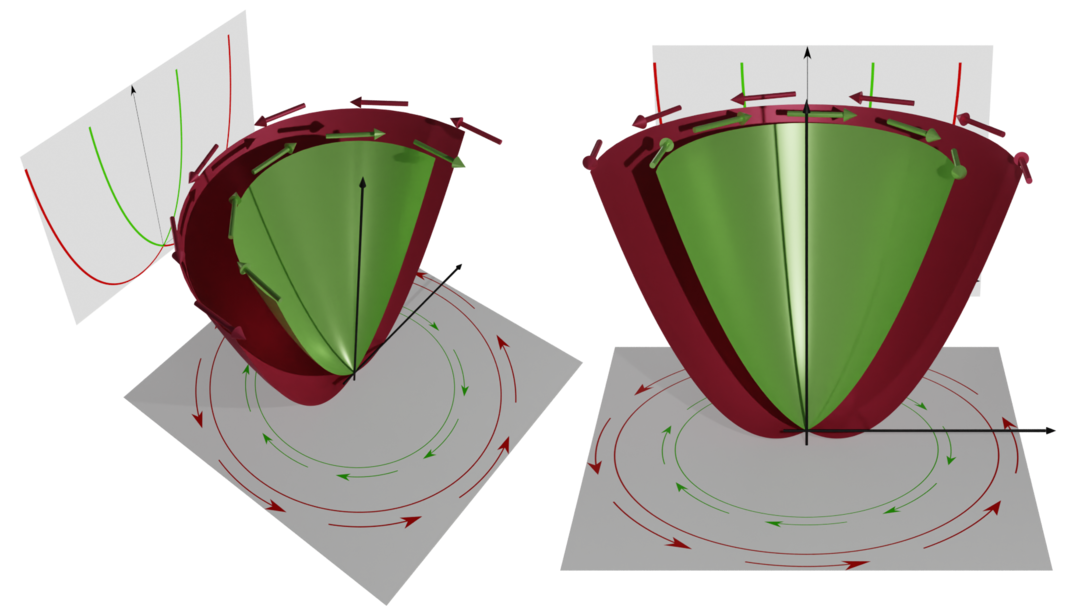
\includegraphics[width=\textwidth]{figures/rashba_combine-wside-small.png}
  \caption{Dispersion curves for a system with Rashba spin-orbit coupling. \textbf{Left:} Seen from above. \textbf{Right:} Seen from the front.
    The projection into the $xy$-plane is shown, as well as a cross section in a plane perpendicular to the $xy$-plane.
    The spin of the two states are shown as arrow above the dispersion curves, which defines the chirality of each state.
    Notice, as is most easily seen in the projection, that the two solutions together form a pair of parabolas separated in momentum.
  }
  \label{fig:rashba}
\end{figure}

% \begin{figure}[ht]
%   \centering
%   \begin{subfigure}[b]{0.48\textwidth}
%     \begin{tikzpicture}
%       \begin{axis} [
%         cycle list name=linestyles,
%         width=\textwidth,
%         ]
%         \addplot {(x-1)^2}
%         node[right]{$\uparrow$};
        
%         \addplot {(x+1)^2}
%         node[right]{$\downarrow$};

%         \draw[<->] (-3, 4) -- (3, 4);
%       \end{axis}
%     \end{tikzpicture}
%     \caption{Band splitting under SoC. Note that Kramer's doublet is not broken.}
%   \end{subfigure}
%   \begin{subfigure}[b]{0.48\textwidth}
%     \begin{tikzpicture}
%       \begin{axis} [
%         cycle list name=linestyles,
%         width=\textwidth,
%         ]
%         \addplot {(x)^2}
%         node[right] {$\uparrow$};
%         \addplot {(x)^2 + 10}
%         node[right] {$\downarrow$};

%         \draw (-3, 4) -- (3, 4);
%       \end{axis}
%     \end{tikzpicture}
%     \caption{Band splitting under Zeeman term. Note the breaking of Kramer's doublet.}
%   \end{subfigure}
%   \caption{Illustration of band splitting when lifting the degeneracy with Zeeman filed and SoC}
% \end{figure}


% \begin{figure}[ht]
%   \centering
%   \ref{named}  %% Legend
%   \begin{tikzpicture}
%     \begin{groupplot}[group style={
%         group name=splitting,
%         group size=2 by 1,
%         horizontal sep=3pt,
%       },
%       xmin=-5, xmax=5,
%       legend to name=named,
%       cycle list name=linestyles,
%       ]
%       \nextgroupplot
%       \addplot {(x-1)^2}
%       node[left]{$\uparrow$};

%       \addplot {(x+1)^2}
%       node[left]{$\downarrow$};

%       \draw[<->] (-3, 4) node[above]{$\downarrow$} -- (3, 4) node[above] {$\uparrow$};
%       \draw[very thin, gray, dotted] (0, -10) -- (0, 40);

%       \nextgroupplot[yticklabels={}]
%       \addplot {(x)^2}
%       node[left] {$\uparrow$};
%       \addplot {(x)^2 + 10}
%       node[left] {$\downarrow$};

%       \draw[<->] (-3, 3^2) node[above]{$\uparrow$} -- (3, 3^2) node[above]{$\uparrow$};
%       \draw[very thin, gray, dotted] (0, -10) -- (0, 40);

%       \legend{$\uparrow$, $\downarrow$}
%     \end{groupplot}
%   \end{tikzpicture}
%   \caption{Illustration of band splitting when lifting the degeneracy with Zeeman filed and SoC.
%     For the SoC (left) Kramer's doublet is not broken. That is, there is an energy degeneracy with opposite spins and momentum.
%     %\todo{find out if this is the actual definiton of Kramer's doublet}
%     For the Zeeman case (right) Kramer's doublet is broken.}
% \end{figure}
